\subsubsection{\textit{Trello}}

O \textit{Trello} é uma ferramenta de gerenciamento de projetos que tem por finalidade auxiliar os líderes de projetos a organizar da melhor forma o fluxo de tarefas relacionadas ao seu trabalho. Utilizando o método \textit{Kanban}, todas as atividades disponibilizadas no \textit{Trello} são exibidas em um único ambiente de trabalho visível por todos os membros da equipe que foram adicionados a ele. As organizações das atividades são feitas através de \textit{cards} (cartões), onde cada membro fica responsável por exercer a atividade que lhe foi designada. O \textit{Trello } possui uma interface bastante amigável e simples de entender \cite{TRELLO2017}. 

Por ser uma aplicação \textit{Web}, o \textit{Trello} necessita de uma conexão com a internet para que os trabalhos possam ser compartilhados e disponibilizados para toda a equipe. A aplicação disponibiliza grandes possibilidades de organização, como por exemplo a criação de atividades distintas dentro de um mesmo projeto, classificação das atividades com rótulo de cores (urgente, não urgente, pouco urgente, descartar, etc), definir a situação de cada atividade (concluída, a fazer, fazendo, etc), dentre outras. Outra grande utilidade que o \textit{Trello} disponibiliza são as notificações por e-mail, que informa a todos os membros a situação de suas atividades dentro do projeto, bem como seu \textit{status}, prazo e níveis de urgência.

A \autoref{fig_trello} apresenta a estrutura de organização deste projeto feita no \textit{Trello}.

\begin{figure}[h]
	\caption{\label{fig_trello}Estrutura organizacional deste projeto feita no \textit{Trello}.}
	\begin{center}
		\resizebox{1\linewidth}{!}{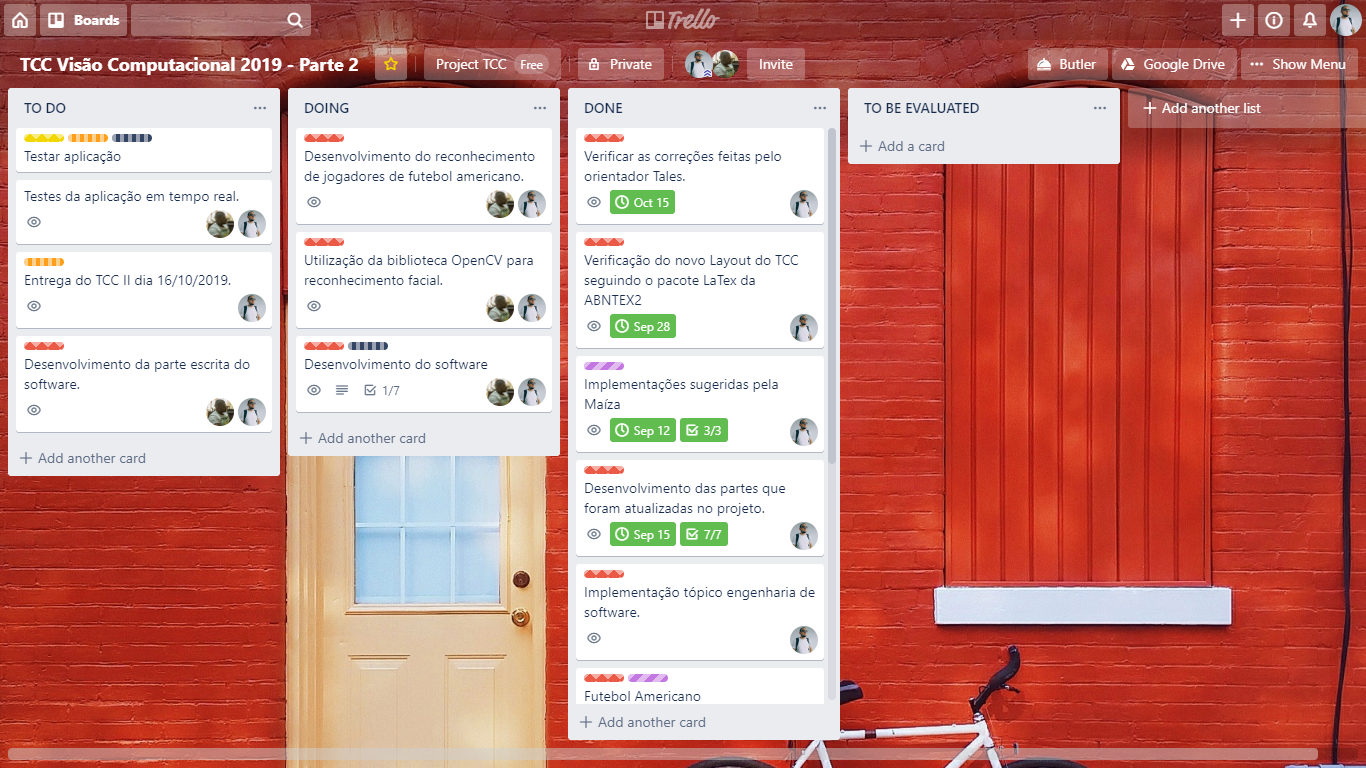
\includegraphics{4-Conteudo-Bibliografico/3-Engenharia-Software/trello.png}}
	\end{center}
	\centering \legend{Fonte: Elaborada pelos autores.}
\end{figure}